\documentclass[12pt,twoside]{article}
\usepackage{booktabs}
\usepackage{jmlda}
\English
\selectlanguage{english}\useshorthands{"}
\title
%    [Нелинейное ранжирование результатов разведочного информационного поиска] % Краткое название; не нужно, если полное название влезает в~колонтитул
{Quality prediction of proteins models with spherical convolutions on three-dimensional graphs}
\author
%    [Мамонов~К.\,Р.] % список авторов для колонтитула; не нужен, если основной список влезает в колонтитул
{Nikita Pavlichenko$^1$, Sergei Grudinin$^2$, Ilia Igashov$^{1,2}$.} % основной список авторов, выводимый в оглавление
%[Мамонов~К.\,Р.$^1$, Воронцов~К.\,В.$^1$, Еремеев~М.\,А.$^1$] % список авторов, выводимый в заголовок; не нужен, если он не отличается от основного
%\thanks
%    {Работа выполнена при финансовой поддержке РФФИ, проект \No\,00-00-00000.
%   Научный руководитель:  Стрижов~В.\,В.
%{Задачу поставил:  Воронцов~К.\,В.
%	 Консультант:  Еремеев~М.\,А.}
\email
{pavlichenko.nv@phystech.edu, sergei.grudinin@inria.fr, igashov.i@yandex.ru}
\organization
{$^1$ Moscow Institute of Physics and Technology, 141701 Dolgoprudniy, Russia;

$^2$ Univ. Grenoble Alpes, Inria, CNRS, Grenoble INP, LJK, 38000 Grenoble, France}%; $^2$Организация}
\abstract
{Convolutional neural networks have become very popular in recent years, and, in particular, have found widespread application in computer
vision. Recently, active work has also begun on graph convolutional networks. In general, the graphs, unlike the pictures, are irregular
structures, and in many tasks of learning on graphs sample objects also do not have unified topology. Therefore, the existing operations
of convolution on the graphs are very much simplified, and the task of pulling on the graphs remain open in general. The purpose of this
work is to research new operations of convolution on three-dimensional graphs within the framework of solving the problem of quality
estimation of three-dimensional models of proteins (the problem of regression on the graph nodes). These operations are theoretical mechanics
inspired methods based on the expansion of a function of spherical coordinates as a linear combination of spherical harmonics. It helps
solve the problem of capturing some local 3D structure of protein residues.
	
	\bigskip
	\textbf{Key words}: \emph {graph convolutional networks, spherical convlutions, three-dimensional graphs learning}.}
\titleEng
{Quality prediction of proteins models with spherical convolutions on three-dimensional graphs}
\authorEng
{Author~F.\,S.$^1$, CoAuthor~F.\,S.$^2$, Name~F.\,S.$^2$}
\organizationEng
{$^1$Moscow Institute of Physics and Technolgy, Moscow, Russia;}
\abstractEng
{This document is an example of paper prepared with \LaTeXe\
	typesetting system and style file \texttt{jmlda.sty}.
	
	\bigskip
	\textbf{Keywords}: \emph{keyword, keyword, more keywords}.}
\begin{document}
	
	\maketitle
	
	\section{Introduction}
	Protein molecules are an important part of any biological form. They determine cellular 
	functions and behavior of various biological and chemical structures. It makes the discovery 
	and prediction of proteins structure one of the most important points of medical, chemical 
	and genetic science researches.

	Molecules of proteins consist of smaller molecules called amino acids. These amino acids
	form a chain that is folded and placed in space. Thus, protein functions are determined
	by their positions in a 3D space. So, having this chain of amino acids we need to identify
	how they are located. There are ways to do this experimentally, but it can be time-consuming,
	expensive, and not always possible. To solve these disadvantages, computational algorithms \cite{Arnold2005}\cite{Lundstroem2008}\cite{Xu2019}
	were developed that generate different chain foldings. The problem is that no algorithm is the 
	best one. Some of the proteins are better modeled by one algorithm, others by others. Therefore, we 
	are facing the problem of quality assessment (QA) of these protein models.

	This problem has recently got attention from the machine learning community. Various artificial
	intelligence methods were applied such as neural networks \cite{Wallner2003} and support vector machines \cite{Ray2012}\cite{Uziela2016}.
	More recent approaches mostly include deep learning methods \cite{Hurtado2018}\cite{Derevyanko2018}\cite{Pages2019}\cite{Conover2019}. The newest approach is to use graph
	machine learning methods such as Graph Convolutional Networks (GCN) \cite{Baldassarre2020GRAPHQAPM}, where the protein is in some
	way represented as a graph. This work brings the new idea of capturing the 3D structure of this graph 
	to improve the quality of GCN using convolutions based on spherical harmonics.


	\section{Problem statement}
	Consider a 3D model of a protein in space. The protein represents a chain of amino acids rolled up in space. 
	Through dividing space around a protein into cells, for example, by the Voronoi method, we can get a
	3D-graph, the vertices of which are amino acids of protein, and edges are carried out between those amino
	acids that are in adjacent cells. Denote the resulting graph by $G = (V, E)$, where verticles $V = (v_1, \ldots, v_n)$
	are a set of amino acids, $E$ are edges. For the $i$-th vertex, we denote for $\mathcal{N}(v_i)$ the
	set of its neighbors in a graph $G$ and for $G$ an adjacency matrix $\boldsymbol{A}$:
	$$A_{ij} = \begin{cases}
		1, & (v_i, v_j) \in E \\
		0, & \text{otherwise}.
	\end{cases}$$ 

	Consider that each vertex $v_i$ is described by some real $d$-dimensional vector of attributes 
	$x(v_i) = \boldsymbol{x}_i$. In the simplest case, it can be a one-hot representation of an amino acid type.
	We can form feature matrix $\boldsymbol{X}$ from vectors $x(v_i)$ for every vertex $x_i$.
	Using these data we will solve a regression problem: to predict for each vertex $v_i$ a real number - its
	"score". In other words, how correctly it is placed in the given 3D-model in comparison with the 
	actual conformation of this protein.

	\section{Graph Convolutional Networks}
	We will develop an approach for machine learning on graphs using Graph Convolutional Network (GCN) \cite{Kipf2016}.
	The idea of this approach is an aggregation of neighbor features for every vertex and forming new feature vectors on the
	layer's output. So, for GCN with $L$ layers, $L \geqslant 2$ we have:
	$$A_{ij} = \begin{cases}
		\boldsymbol{H}^{(0)} = \boldsymbol{X} \\
		\boldsymbol{H}^{(l)} = \sigma\left(\boldsymbol{A} \boldsymbol{H}^{l-1}\boldsymbol{W}^{(l-1)}\right) & \text{for } l \in \{1, \ldots, L - 1\} \\
		\boldsymbol{H}^{(L)} =  \boldsymbol{A} \boldsymbol{H}^{L-1}\boldsymbol{W}^{(L-1)}.
	\end{cases}$$
	In the above $\boldsymbol{H}^{(l)}$ denotes feature matrix at $l$-th layer and $\boldsymbol{W}^{(l)}$ denotes weight matrix. Common choice for activation
	function $\sigma$ is a ReLU activation: $\text{ReLU}(x) := \max(x, 0)$ or an ELU activation: $\text{ELU}(x) := \begin{cases}
		x, & x \geqslant 0 \\
		\alpha(e^x - 1), & x < 0
	\end{cases}$.
	Weights matrix $\boldsymbol{W}^{(l)}$ are trained by stochastic gradient descent or its modifications.

	We rely on this approach because it has already shown outperformance in the protein quality
	 assessment problem\cite{Baldassarre2020GRAPHQAPM}.
	
	The main problem here is that classic GCN is not able to use information about locations of vertices in space. This is because the coordinates in space
	are given ambiguously: the turned or shifted proteins are actually isomorphic. So our improvement is to capture such information from
	the sequential structure of a protein.

	\section{Spherical Convolutional Networks}
	\subsection{Spherical harmonics}
	Let us consider a function $f(\Omega) : [0, \pi] \times [0, 2\pi) \rightarrow \mathbb{R}$ — mapping from unit sphere to real
	numbers. That function might be unknown or its evaluation might be time-consuming. So, we want to expand this function as a linear
	combination of simpler functions. The common approach that came from theoretical mechanics is to use spherical harmonics\cite{Mueller1966}.
	We will use the following form of spherical functions:
	$$
		Y_l^m(\phi, \psi) = \sqrt{\dfrac{(2l + 1)}{4\pi}\dfrac{(l-m)!}{(l+m)!}}P_l^m(\cos \phi)e^{im\psi}, 
	$$
	where $P_l^{m}$ are associated Legendre polynomials\cite{Mueller1966}.

	On the unit sphere, any square-integrable function can thus be expanded as a linear combination of these:
	$$
	f(\phi, \psi) = \sum_{l = 0}^{\infty} \sum_{m=-l}^{m=l}f_l^m Y_l^m(\phi, \psi).
	$$
	We will use this fact to train a function of vertex features using the first few components of this expansion. 
	Since the function is real, the real representation of spherical harmonics can be used:
	$$
	Y_{lm} = \begin{cases}
		\sqrt{2}(-1)^m \Im\left[Y_l^{|m|}\right] & \text{if } m < 0 \\
		Y_l^0 & m = 0 \\
		\sqrt{2}(-1)^m \Re\left[Y_l^{m}\right] & \text{if } m > 0.
	\end{cases}
	$$

	\subsection{Spherical convolution}
	Consider a vertex $v_i$. Since all the amino acids in the protein are connected in a peptide chain, it is easy to
	construct its local coordinate system for the amino acid $v_i$ under consideration — on two dihedral corners,
	which are unambiguously determined from the geometry of the peptide chain. Write the coordinates of all the neighbors of $v_j \in \mathcal{N}(v_i)$
	of the amino acid in the obtained coordinate system. Then proceed to spherical coordinates, and project all vertices onto a unit sphere
	with the center in $v_i$. Now, each vertex $v_j \in \mathcal{N}(v_i)$ can be matched with a pair of angles $\Omega_i^j = (\phi_i^j, \psi_i^j)$ that specify the
	angular position of the projection of the vertex $v_j$ onto a unit sphere in the local coordinate system of $v_i$.

	Now, having an unambiguous orientation for each vertex of the graph, we can introduce the convolution operation. Let us consider a certain 
	matrix function $f(\Omega) : [0, \pi] \times [0, 2\pi) \rightarrow \mathbb{R}^{d \times d'} $ on a single sphere. We can expand it
	into a series on the basis of spherical functions $\{Y_l^m\}_{l,m}$ and leave the first few components:
	$$
		f(\Omega) \approx f_W(\Omega) = \sum_{l=0}^{L}\sum_m \boldsymbol{W}_l^m Y_l^m(\Omega),
	$$
	where $\boldsymbol{W}_l^m$ denotes coefficient matrix in the expansion of matrix function $f$ on the basis of $\{Y_l^m\}_{l,m}$. Then
	we can introduce the spherical convolution operation for the vertex $v_i$ in the following way:
	$$f_W \circ v_i = \sum_{v_j \in \mathcal{N}(v_i)} f_W(\Omega_i^j)x(v_i).$$

	Considering $\boldsymbol{W}_l^m$ matrices to be optimized parameters, we will thus train spherical filters.

	\subsection{Spherical convolution layer}
	Let us have a 3D model of a protein consisting of $N$ amino acids, the $i$-th amino acid is described by the trait vector $\boldsymbol{x}_i \in \mathbb{R}^d$.
	Let us denote all the vertices through the $\boldsymbol{X} \in \mathbb{R}^{N \times d}$ feature matrix. Then one layer of spherical
	convolution is written down as follows:
	$$
		\boldsymbol{X} \longrightarrow \boldsymbol{X}' = \sigma(f_W \circ \boldsymbol{X}) = \sigma\left(\sum_{l,m}Y_l^m(\boldsymbol{A}_\Omega)\boldsymbol{X}\boldsymbol{W}_l^m\right),
	$$
	where $\sigma$ is an activation function, $Y_l^m$ are spherical functions, $\boldsymbol{W}_l^m$ are optimized parameters and $\boldsymbol{A}_\Omega$
	is the adjacency matrix of graph $G$, which cells contain the spherical coordinates of the vertices in the corresponding local coordinate system:
	$$
		[\boldsymbol{A}_\Omega]_{i,j} = \begin{cases}
			\Omega_i^j, & (v_i, v_j) \in E \\
			0 & \text{otherwise}.
		\end{cases}
	$$

	\section{Experiment}
	\subsection{Dataset}
	All models are taken from the CASP competition data (\url{http://predictioncenter.org}), which is dedicated to the prediction 
	of the 3D structure of proteins by the amino acid sequence. We take data from CASP12 and CASP13 as a test sample and data from
	earlier CASPs as a training sample.

	For each protein, there is one real experimentally obtained 3D structure and many generated 3D structures. Our task is to predict 
	the CAD-score \cite{Olechnovic2012} for each of the generated structures i.e. how similar each of the generated structures is to the real one.
	Graphs are generated using Voronoi diagrams with weights — an area of contact.

	We have precalculated spherical harmonic of the order of $5$ for every pair of incident residues. This took 60GB of HDD space when
	calculated on CASP8-CASP12. So, it appears to be the main problem there, comparing to the fact that raw data takes only
	15GB and that value grows as $n^2$, where $n$ is an order of spherical harmonic.

	\subsection{Metrics}
	In this task, there is a problem of selecting the right quality metric. It was found that MSE's conventional metric used
	for training was not suitable for evaluating the quality of the algorithm. This is due to the fact that it does not 
	reflect what the algorithm was created for at all — to select protein folding models. So, we need a more suitable metric.
	Often Pearson correlation between CAD models or residues and algorithm predictions is chosen for this purpose\cite{Baldassarre2020GRAPHQAPM}.
	We will also use a \textbf{z-score} metric because it represents how good is the model with the
	maximum predicted score.

	We will calculate these metrics for every protein, and then average them. As a result, we will get the global metric value.

	\subsection{Baseline}
	For the baseline, we will use an architecture inspired by GraphQA\cite{Baldassarre2020GRAPHQAPM} network. Firstly, we encode residues features
	to high-dimensional space using linear layers with size increasing by a power of two. For the next step, we process obtained features through
	8 graph convolutional layers to account for the relationships of residues. Finally, we pass the result through a multi-layer perceptron and get
	single output with a sigmoid activation function as the CAD score is from 0 to 1. We have chosen ELU as an activation function for hidden layers.
	Adam optimizer\cite{Kingma2014} is used for training with a learning rate set to $0.001$.

	This model was trained on CASP8, CASP9, CASP10, CASP11 datasets for 50 iterations and evaluated on CASP12. We decided to train
	it on CPU because the slowest part of the training was the loading features and adjacency matrices from HDD.
	\begin{figure}[H]
		\centering
		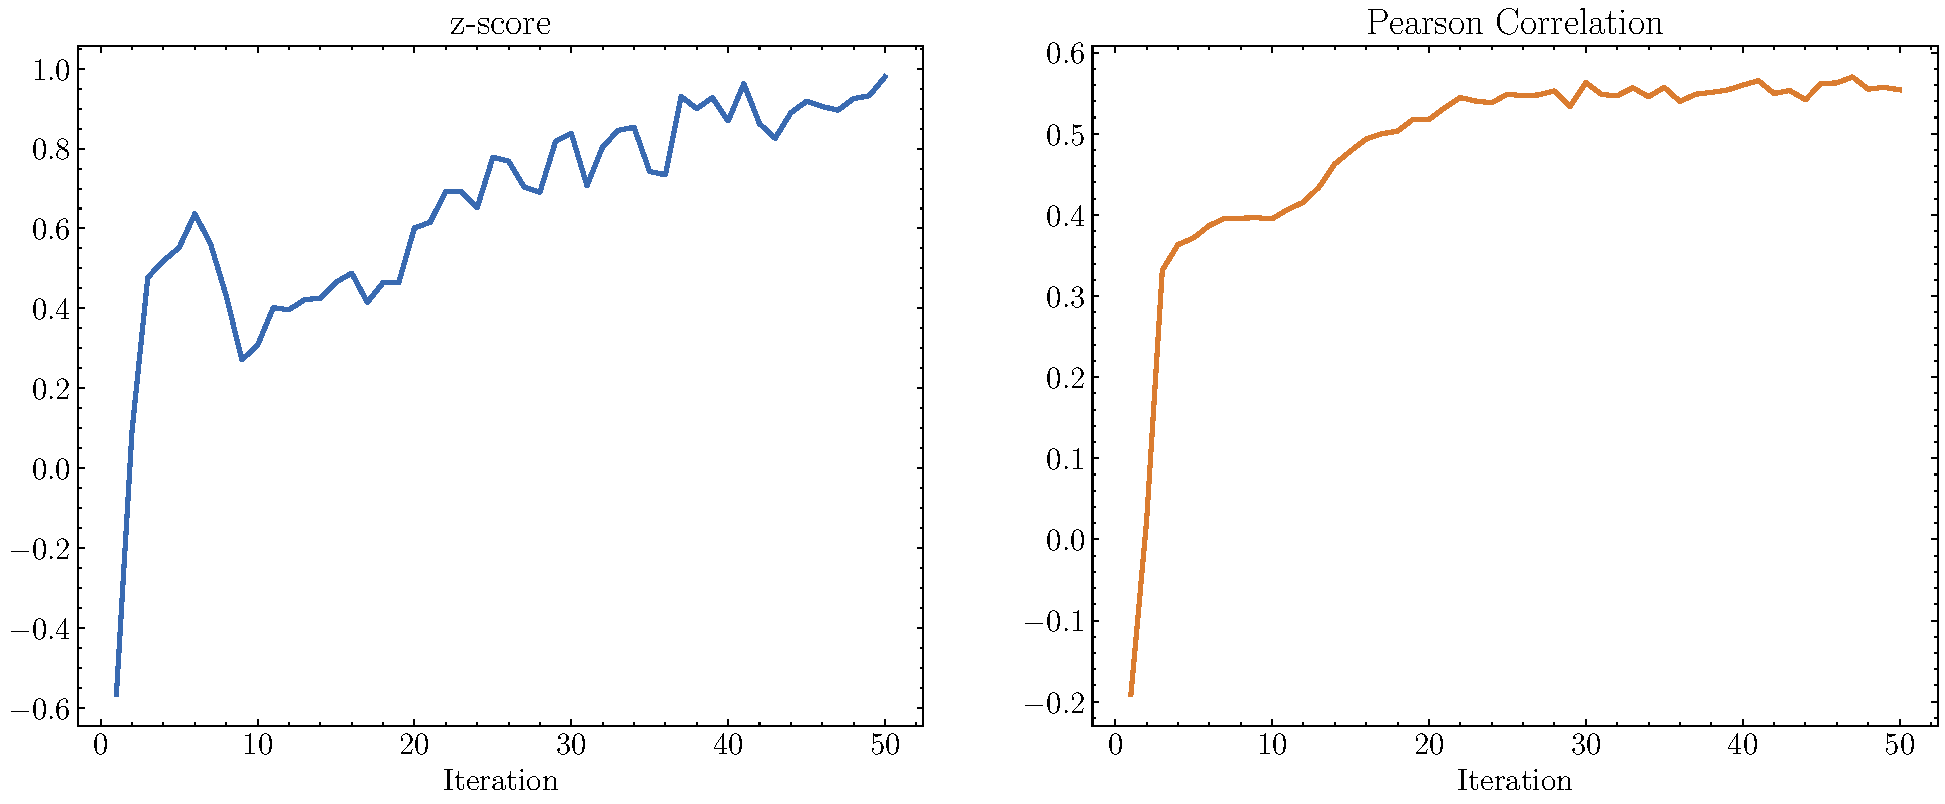
\includegraphics[width=1.0\textwidth]{img/z_score_casp12.pdf}
		\caption{z-score and Pearson and Spearman correlation coeffients for each iteration on CASP12 dataset of baseline 
		GCN.}
		\label{fig:mesh1}
	\end{figure}

	We managed to achieve the maximum Pearson correlation value of $0.57$ and the maximum z-score value of $0.979$. It is significantly lower
	than many state-of-the-art algorithms\cite{Baldassarre2020GRAPHQAPM} but it can be explained by the fact that we only used the geometric structure of proteins.
	All the high results were obtained only with the use of complex features that represent chemical relations between residues and some
	biological features that represent protein evolution\cite{Baldassarre2020GRAPHQAPM}.

	\subsection{Spherical Convolutional Networks}
	We have run the same architecture with spherical convolutional layers instead of GCN. The main problem there was the fact, that
	the number of trained parameters has increased in $25$ times because we have used spherical harmonics of the order of $5$. So, we
	have decreased the learning rate and started learning on GPU because the loading from HDD now is not a bottleneck.
	\begin{figure}[h]
		\centering
		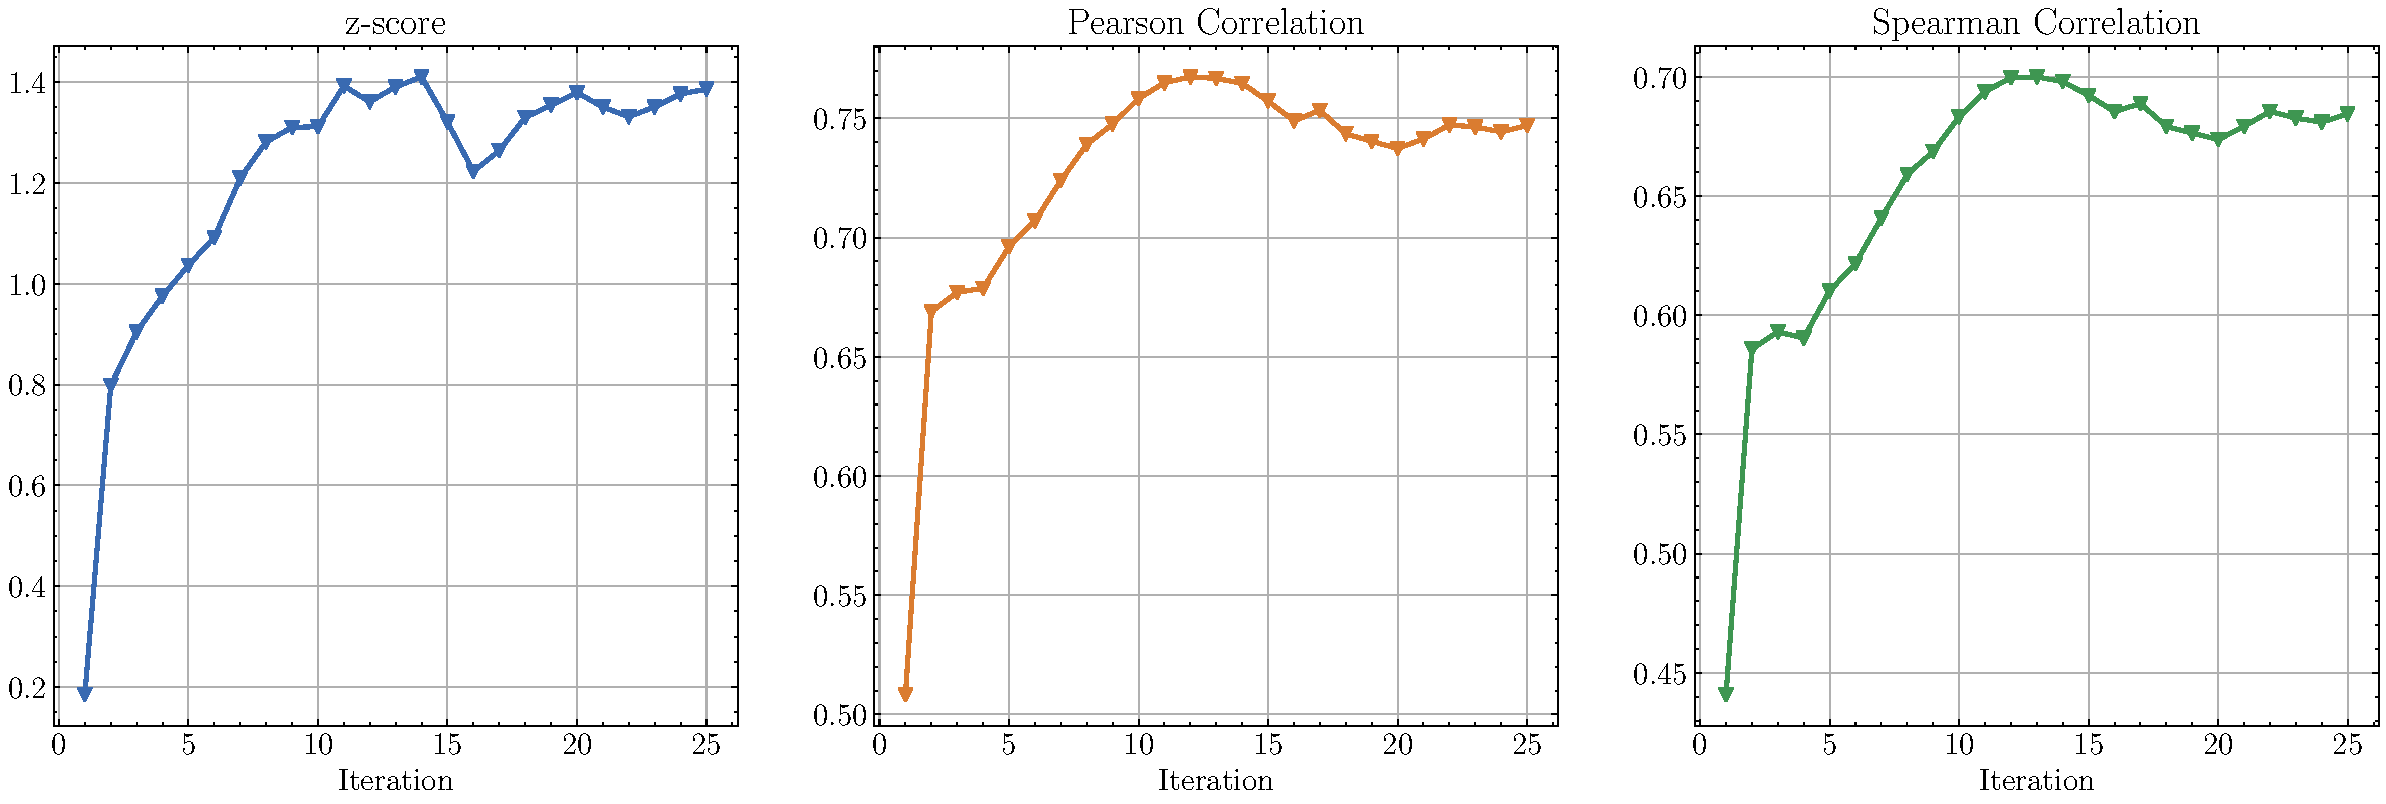
\includegraphics[width=1.0\textwidth]{img/z_score_casp12_sh.pdf}
		\caption{z-score and Pearson and Spearman correlation coeffients for each iteration on CASP12 dataset of SCN.}
		\label{fig:mesh1}
	\end{figure}

	\subsection{Comparsion}
	Table 1 the performance of state-of-the-art methods of Protein Quality Assessment. The important remark there is
	the fact that other approaches shown in this table use biological and chemical features but in turn, we use only the geometric representation
	of residues graph. Despite that fact, Spherical Convolutional Network has shown high performance.
	\begin{center}
		\begin{table}[H]
			\centering
			\begin{tabular}{l|l|l|l|l}
				\hline
					   & $\rho$ &  $r$     &   rank       & z-score \\ \hline
			ProQ3D     & 0.801  &  0.750   &   11.961     & 1.670       \\
			VoroMQA    & 0.803  &  0.766   &   17.171     & 1.410       \\  
			SBROD      & 0.685  &  0.762   &   23.579     & 1.282       \\
			Ornate     & 0.828  &  0.781   &   10.776     & 1.780       \\
			Simple GCN & 0.570  &  0.510   &   31.667     & 0.979       \\
			SCN        & 0.767  &  0.700   &   18.462     & 1.411       
		\end{tabular}
		\caption{Comparsion of Pearson, Spearman correlation coefficients and z-score and rank of the state-of-the-art algorithms,
			our GCN baseline and Spherical Convolutional Network on CASP12 dataset.
			}
		\label{Tab:1}
		\end{table}
	\end{center}

	We see that Spherical Convolutional Network has shown significantly better performance than GCN. It shows that our approach
	is applicable and appears to be an improvement to Graph Convolutional Networks.

	\begin{figure}[h]
		\centering
		\includegraphics[width=1.0\textwidth]{img/dist_casp12_scn.pdf}
		\caption{Distribution of SCN scores on target structures and models from CASP12. Solid lines represent kernel density estimations of the corresponding distributions.
		}
		\label{fig:mesh1}
	\end{figure}

	\section{Conclusion}
	For the first time, we applied spherical convolutions for capturing the 3D structure of the graph. The results have shown that it could
	give significant improvement in the quality of the algorithm. This idea can be combined with other ideas introduced in other papers
	\cite{Pages2019}\cite{Baldassarre2020GRAPHQAPM}\cite{Uziela2016} so we hope that it can achieve even higher results in the problem
	of Protein Quality Assessment. We want to notice that the idea of spherical convolutions is universal and can be applied to
	various types of tasks of learning on graphs with 3D structure and hope that it will find such applications.

	Finally, we wish that this idea will be developed and be applied in more complicated approaches of learning on graphs such as
	graph variational autoencoders\cite{Kipf2016a} and Quality Assessment will become a popular task in the machine learning community.
	%\begin{State}
	%    Мотивации и~интерпретации наиболее важны для понимания сути работы.
	%\end{State}
	
	%\begin{Theorem}
	%    Не~менее $90\%$ коллег, заинтересовавшихся Вашей статьёй,
	%    прочитают в~ней не~более~$10\%$ текста.
	%\end{Theorem}
	%
	%\begin{Proof}
	%    Причём это будут именно те~разделы, которые не содержат формул.
	%\end{Proof}
	%
	%\begin{Remark}
	%    Выше показано применение окружений
	%    Def, Theorem, State, Remark, Proof.
	%\end{Remark}
	
	
	%\section{Заключение}
	
	%Желательно, чтобы этот раздел был, причём он не~должен дословно повторять аннотацию.
	%Обычно здесь отмечают,
	%каких результатов удалось добиться,
	%какие проблемы остались открытыми.
	
	
	\bibliographystyle{plain}
	\bibliography{Pavlichenko2020Project52}
	
	% Решение Программного Комитета:
	%\ACCEPTNOTE
	%\AMENDNOTE
	%\REJECTNOTE
\end{document}
